\documentclass[bare_jrnl_transmag]{subfiles}
\begin{document}
\subsection{Limitations}
From the results of the filter, it is apparent that, while performing better than a pure dead-reckoning approach, the Kalman filter exhibits drift in its position estimation. Figure \ref{fig:dead_reackoning} shows the results of an inertial dead-reckoning approach on the training dataset, demonstrating the improvement offered with the vision-based fusion. The RMSE of the dead-reckoning approach is 7.01, 10.08, and 0.91 meters for x, y, and z respectively.

\begin{figure}[H]
    \centering
    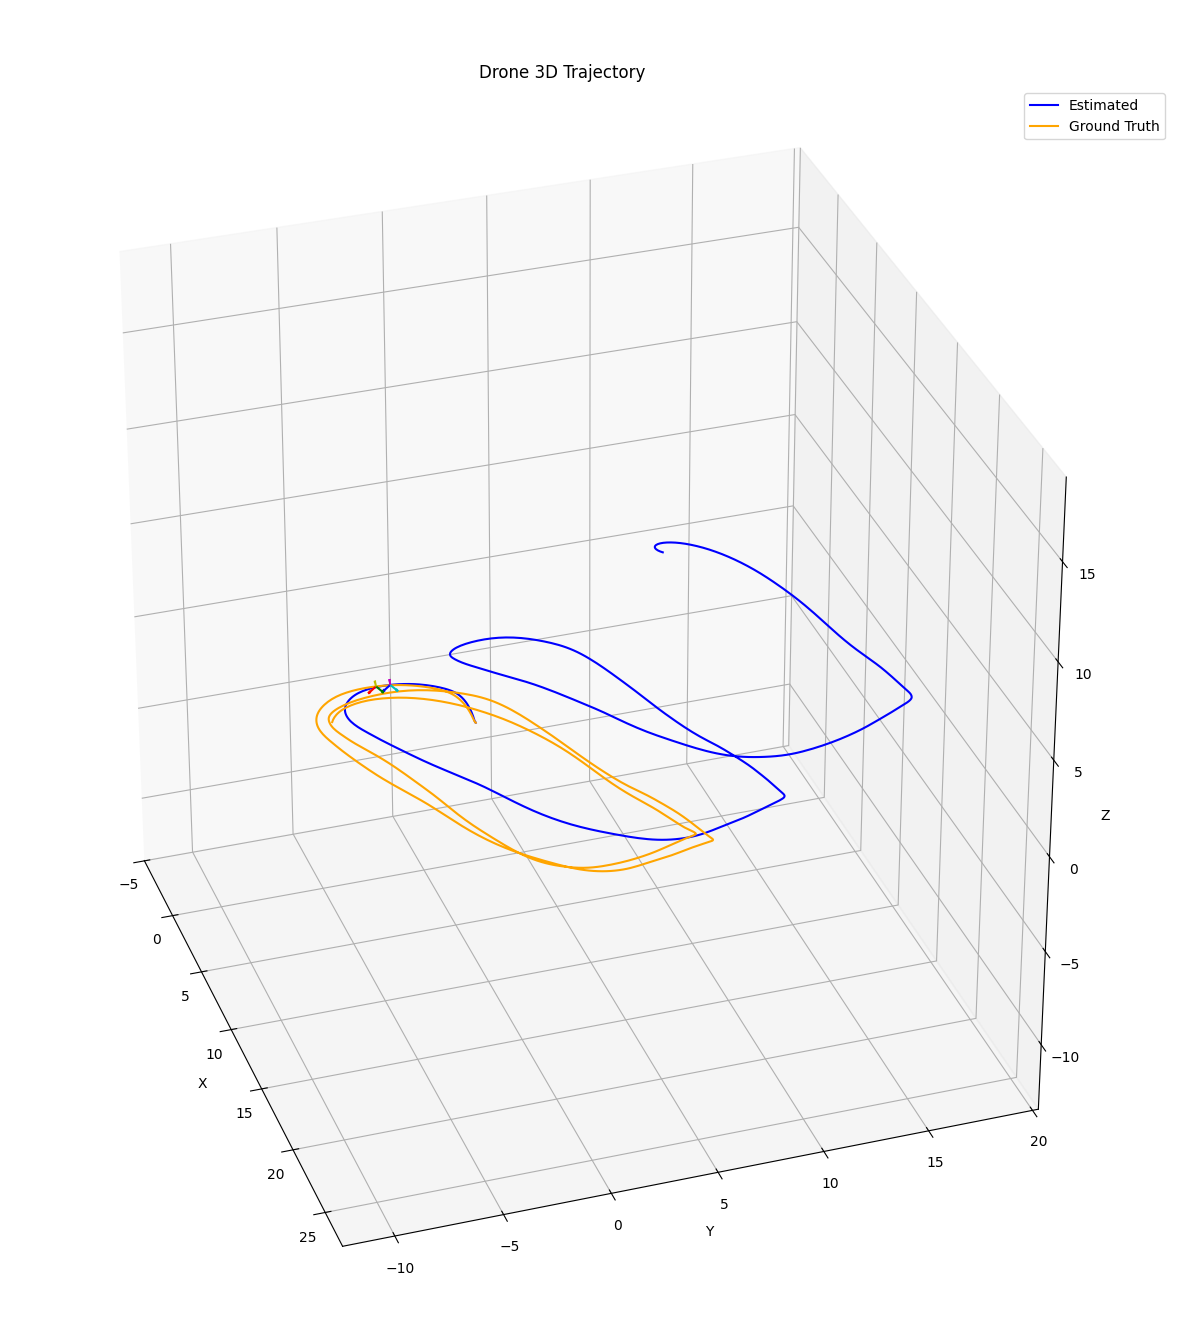
\includegraphics[width=0.8\linewidth]{figures/dead_reckoning_results_training.png}
    \caption{Dead-reckoning results comparing the ground-truth pose of the drone to the estimated pose on the training dataset.}
    \label{fig:dead_reackoning}
\end{figure}

The above figure shows the significant amount of drift that results from a pure dead-reckoning approach in the X/Y plane. The Kalman filter is able to reduce this drift significantly, but it is still present. While the orientation estimation is quite accurate, the Madgwick filter has no way of correcting for yaw drift in the absence of another sensor (ex: magnetometer). As a result, a poor yaw estimate will cause the position estimation to drift, especially as the motion model directly integrates acceleration measurements in the estimated body frame. 

\subsection{Discussion}
As a result of the above limitations, the VIO fused algorithm performed better than a dead-reckoning approach. Strengths of the algorithm include:
\begin{itemize}
    \item Elimination of drift in the X/Y position with camera correction input
    \item Accurate orientation pose estimation in the world frame with the Madgwick filter 
\end{itemize}

Clear limitations of the algorithm include:
\begin{itemize}
    \item Drift in the Z axis introduced by the fusion of the visual odometry algorithm. While the cause of this is unknown, a possible explanation is that the camera is not able to accurately measure the Z axis due to the nature of the stereo camera setup during high speed flight or turning motions. As a result, the VIO algorithm falsely integrates the Z axis acceleration, causing drift. This may be mitigated with further tuning of the VIO algorithm or by adding another sensor (ex: barometer) to correct for Z axis drift.
    \item Yaw drift from the Madgwick filter as run time increases - this may be correctable by employing a magnetometer or with another type of filter that is able to incorporate yaw correction from visual odometry. 
    \item Lack of a robust motion model for the Kalman filter - the current model is a simple constant velocity model, which does not account for acceleration, deceleration, or turning motions. This may be improved with a more complex motion model that is able to account for these factors using interactive multiple model (IMM) filtering or a more complex Kalman filter model.
\end{itemize}



\end{document}